\chapter{Database Design}

\section{Entities, Attributes and Relationships}
The database, called doctor, will have seven tables User, doctor, patient, disease, patientDetails, Medication, appointment. Each table holds details about patient and doctor involved in booking and the details about the patient. The two
tables will be linked through a foreign key. The doctor DataBase will have following details\\

\thispagestyle{fancy}
\section{Functional Requirements}
\subsection{Major Entities}
\textbf{User}: To store the login information and determine patient and doctor login seperately.\\
\textbf{doctor}: To store details of all doctors.\\
\textbf{disease}: To store details of diseases and its type.\\
\textbf{patientDiseases}: To store additional details of the patient.\\
\textbf{appointment}: To store appointment details like patient and doctors involved in the appointment.\\
\textbf{UserFeedback}: To store the opinion of the users about the site.\\
\thispagestyle{fancy}

\section{ER Diagram}
\begin{figure}[H]
    \centering
    \subfloat{{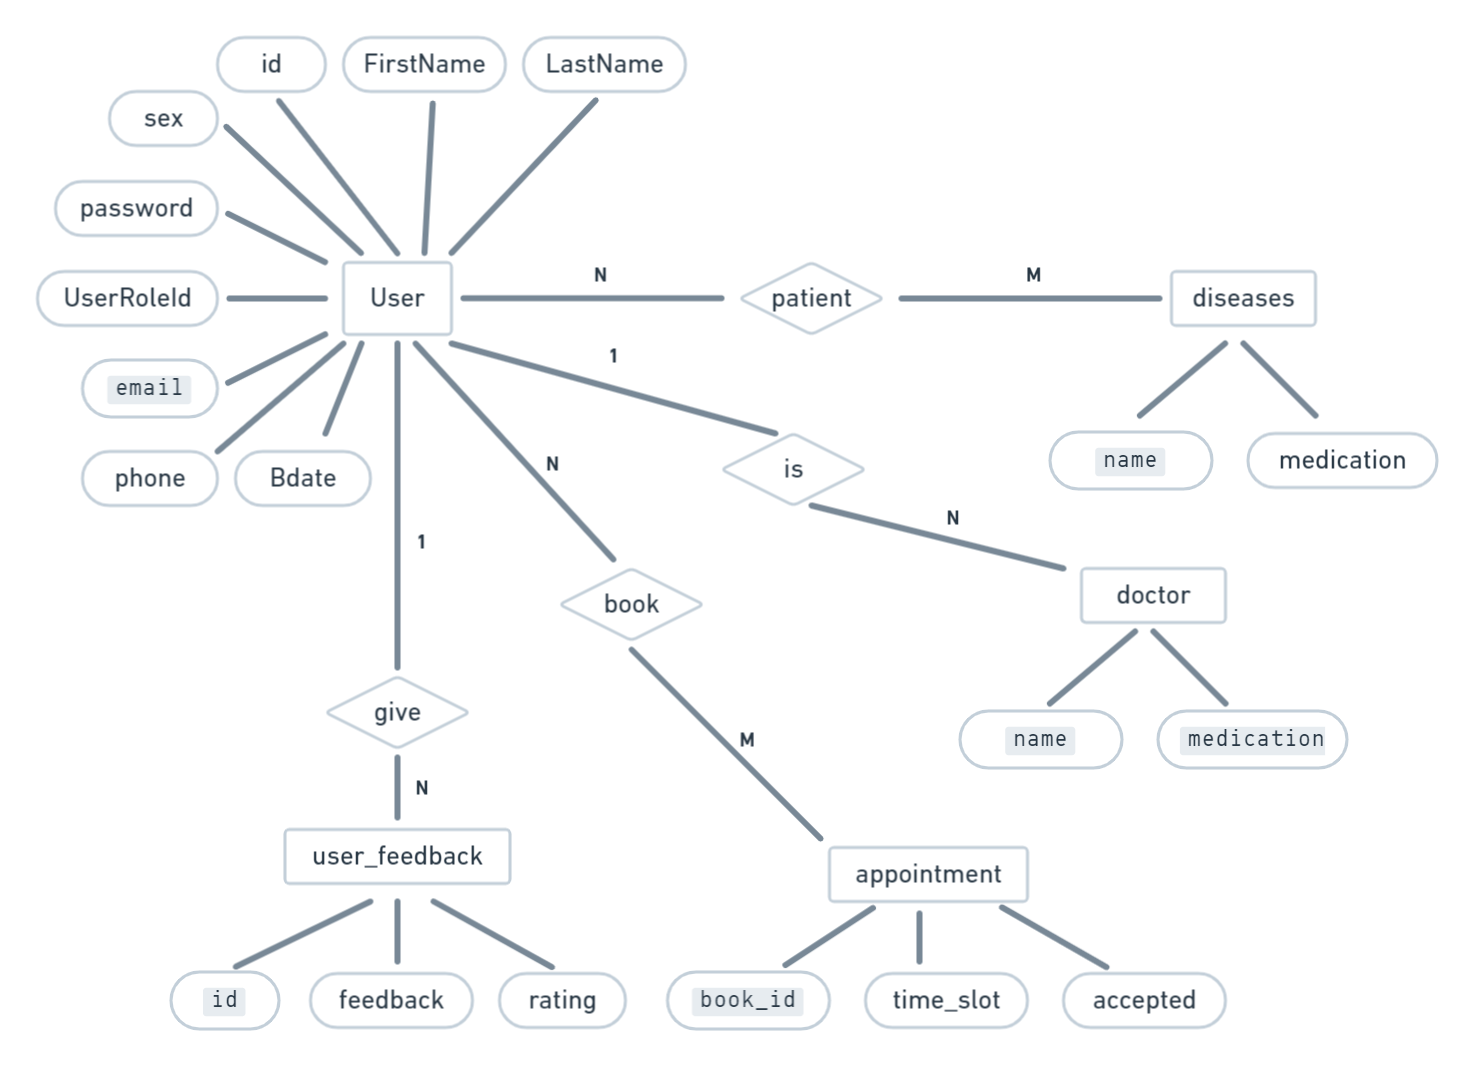
\includegraphics[width = 17cm]{./ERD.png} }}%
    \qquad
    \caption{Entity Relationship Diagram}%
    \\[0.2in]
    \label{fig: Entity Relationship Diagram}
    \centering
\end{figure}

% \pagebreak
\thispagestyle{fancy}

\section{Schema Diagram}
\begin{figure}[H]
    \centering
    \subfloat{{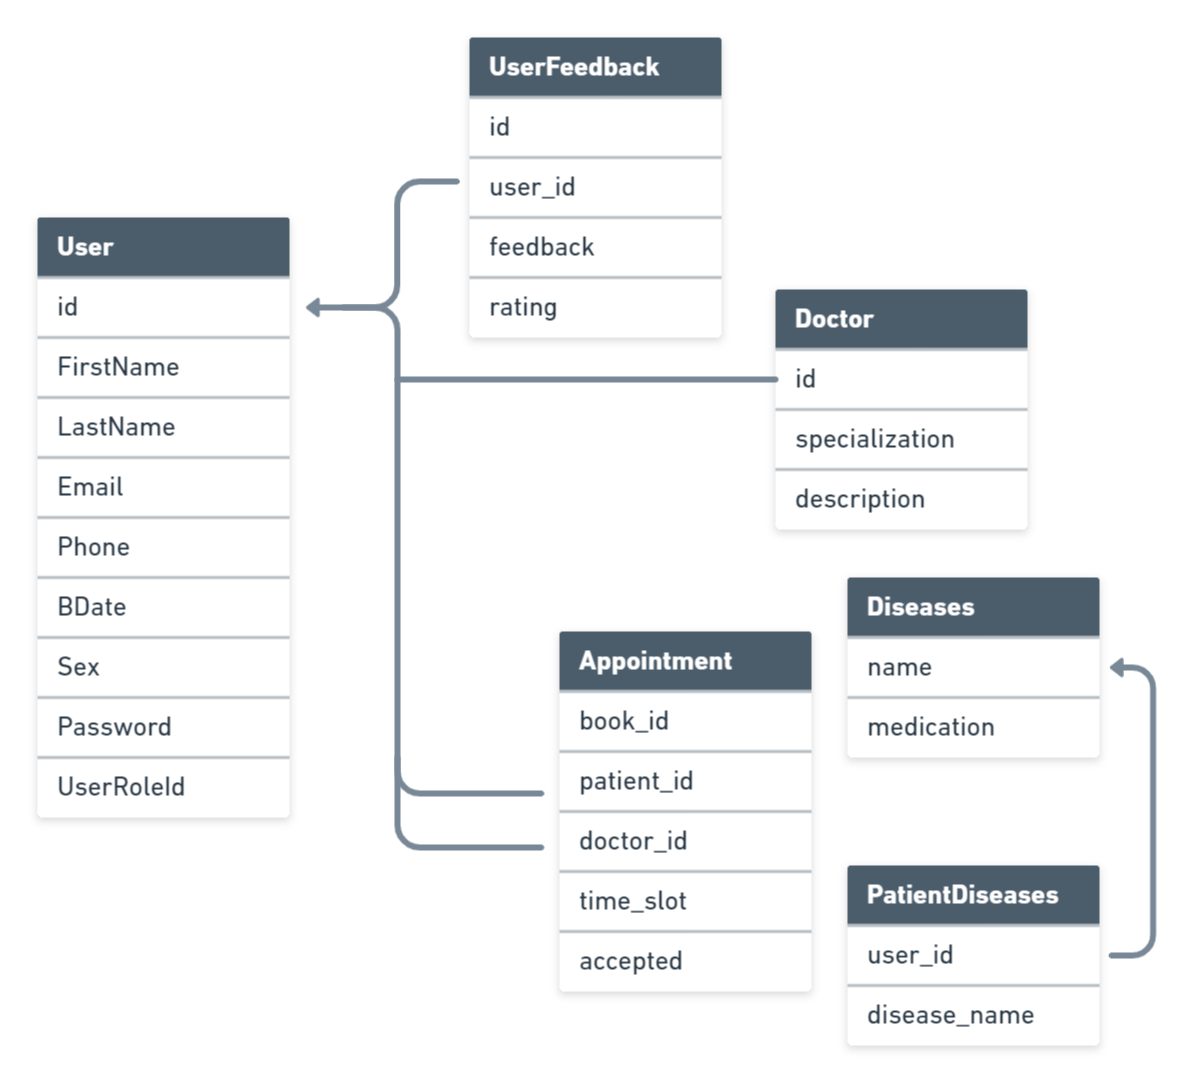
\includegraphics[width = 17cm]{./schema.png} }}%
    \qquad
    \caption{Schema Diagram}%
    \\[0.2in]
    \label{fig: Schema Diagram}
    \centering
\end{figure}
